\newpage
\section{Transform[EK]}\label{sec:transform}
Nachdem alle Datenquellen im Extrakt ihre speziell zugeschnitten Extraktionslösungen erhalten haben, welche die Besonderheiten der Datenquellen berücksichtigen, kann nun die Phase der Transformation eingeleitet werden. In diesem Teil kommen die validierten aber noch nicht nutzbaren Rohdaten an. Dieser Schritt ist auch jener, welcher dem ETL-Prozess eine große Wertschöpfungsmöglichkeit erlaubt, indem die Daten so aufbereitet werden, dass möglichst aussagekräftige BI-Reports daraus erstellt werden können. Damit diese Aufbereitung erfolgreich ablaufen kann, werden die multiplen Rohdatensätze normalisiert und in ein einziges Systemformat gebracht. 
\vspace{5mm}\par
Nicht alle extrahierten Daten benötigen zwingend eine Transformation, solche Daten werden Pass-Through-Daten genannt.
\vspace{5mm}\par
Eine gewisse Komplexität kommt durch Probleme der Datenintegrität auf. So kann es vorkommen, dass bestimmte Daten zusammen gehören, aber einen andere Identifikation tragen. Die Stadt „Vienna“ und „Wien“ bezeichnen den selben Ort, aber in verschiedenen Schreibweisen. Anders kann dies auch vorkommen: Daten tragen eine gleiche Identifikation und gehören so eigentlich nicht zusammen. Zum Beispiel gibt es Städte in der Welt, welche den gleichen Namen tragen, aber auf zwei verschiedenen Kontinenten liegen: Paris in Frankreich ist nicht Paris in Texas. Visuell wird dies nochmals durch die folgende Grafik veranschaulicht:

(vgl. \cite{ETL-Process} \& \cite{ETL-Explained})
\begin{figure}[H]
    \centering
    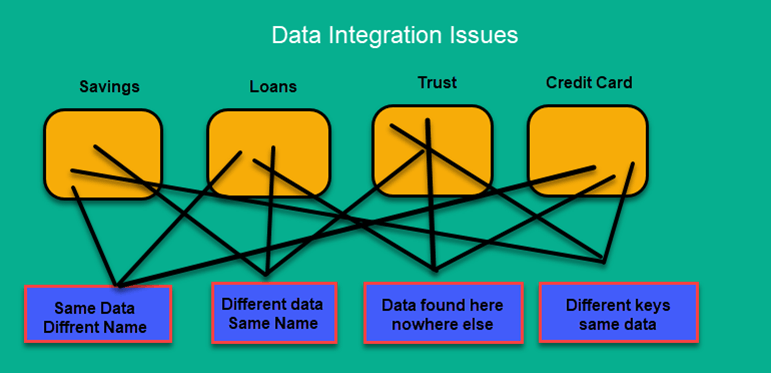
\includegraphics[scale=0.5]{images/etl-integration-issues.png}
    \caption{Probleme der Datenintegration (02.04.2020)}
    \url{https://www.guru99.com/images/1/022218_0848_ETLExtractT2.png}
\end{figure}
\newpage
Es gibt ein Vielzahl von Validationen, welche im Laufe eines Transform-Prozesses auftreten können. Ein paar Beispiele:
\begin{itemize}
    \item Filtern von Daten - nur spezielle Daten sollten an den Load-Prozess übergeben werden
    \item Benötigte Felder sollten keine leeren NULL-Felder enthalten
    \item Maßeinheiten sollten alle in ein bestimmtes Format umgewandelt werden
    \item Die Datensätze sollten nach einem speziellen Kriterium sortiert werden
\end{itemize}
Allgemein lässt sich sagen, dass in die Validation alle Tätigkeiten fallen können, welche die Daten aufbereiten und so besser nutzbar machen. Der Fokus liegt hier, im Unterschied zur eigentlichen Datenanalyse, in der Tatsache, dass noch keine Schlüsse aus diesen Daten gezogen werden sollen, sondern nur dies im späteren Verlauf erleichtert.
\vspace{5mm}\par
Zusammenfassend kann gesagt werden, dass es sich bei der Transformation um einen sehr angepassten Prozess handelt. Somit ist eine große Variation in der Komplexität, je nach Anforderung und Datensets, möglich.
(vgl. \cite{ETL-Process} \& \cite{ETL-Explained})